\documentclass[10pt,a4paper]{article}
\usepackage[utf8]{inputenc}
\usepackage[magyar]{babel}
\usepackage[T1]{fontenc}
\usepackage{amsmath}
\usepackage{amsfonts}
\usepackage{amssymb}
\usepackage{graphicx}
\begin{document}

\section{14. sz. laboratóriumi mérés}
	Mérés dátuma:\date{2017.10.02}
	\subsection{A mérés célja}
	Az ellenállás mérésére használatos néhány módszer alkalmazásának elsajátítása. Igen kis ellenállások nagypontosságú mérése.
A méréseknél előforduló mérési hibák meghatározása.
	\subsection{Mérési feladatok}
		\subsubsection{Feszültség összehasonlító módszerrel határozza meg a 4. sz
mérőpanelen található R7 $= 10 \Omega $ és R4 $= 82 \Omega $ névleges értékű ellenállások pontos értékét és bizonytalanságukat!
A mért és a számított eredményeket foglalja össze táblázatba. A méréseknél
az elérhető legnagyobb pontosságra törekedjék!}
		Mérendő objektum:
		\\\\
		\begin{figure}[hbtp]
		\centering
		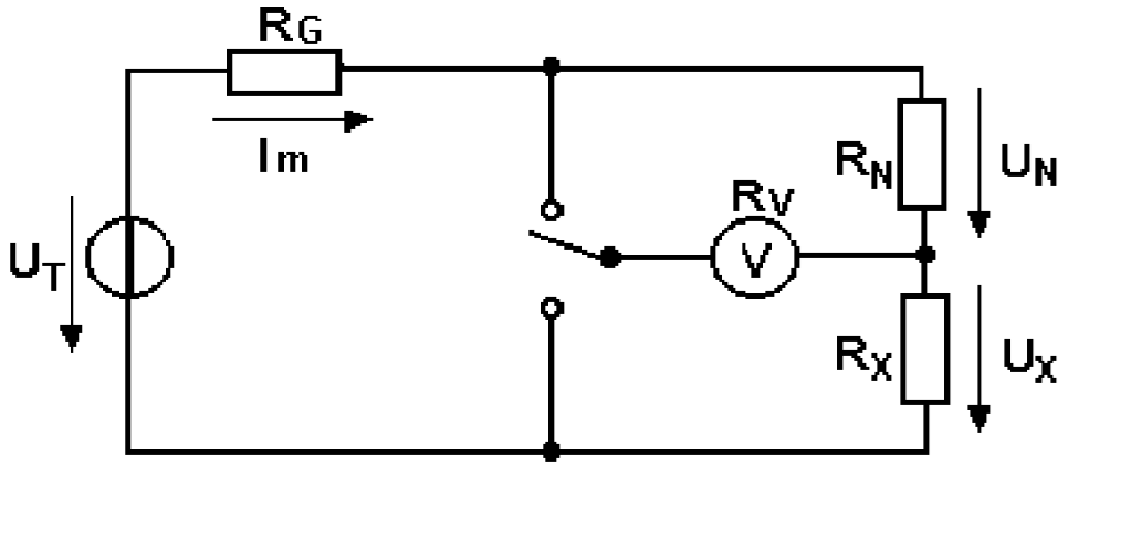
\includegraphics[scale=0.5]{teljes/fesz_ossze.png}
		\caption{Feszültség összehasonlító módszer}
		\end{figure}
		\\\\
		Határadatok: mivel $R_G$ a legnagyobb ellenállás, és mindegyiknek a megengedett maximálisan felvehető teljesítménye $0,25 W$, ezért célszerű $R1 = R_G$ ellenállással a maximális tápfeszültséget meghatározni.
		$$P = I^2_{m} * R$$
		$$I_m = \sqrt{\frac{P}{R}} = \sqrt{\frac{0,25W}{1k\Omega}} = 15,8 mA$$
		$$U_{Tmax} = \frac{I_m * R_G}{3} = \frac{15,8 mA * 1 k\Omega}{3} = 5 V$$
		Mért értékek:\\\\
		\begin{tabular}{|c|c|c|}
		\hline 
		$R_x$ & $R_4$ & $R_7$ \\ 
		\hline 
		$U_N$ &  &  \\ 
		\hline 
		$U_X$ &  &  \\ 
		\hline 
		$R_{valodi}$ & - &  \\ 
		\hline 
		\end{tabular} 
		\\\\ 
		
		Hibaszámítás (HM8012):\\\\
		
		$$$$ $$$$
		\subsubsection{Áramösszehasonlító módszerrel határozza meg a 4. sz mérőpanelen
található R15 $= 100 k\Omega$ névleges értékű, valamint az R11 ismeretlen értékű
ellenállásokat és bizonytalanságukat! A mért és a számított eredményeket
foglalja össze táblázatba. A méréseknél az elérhető legnagyobb pontosságra
törekedjék!
}		Mérendő objektum:
		\\\\\begin{figure}[hbtp]
		\centering
		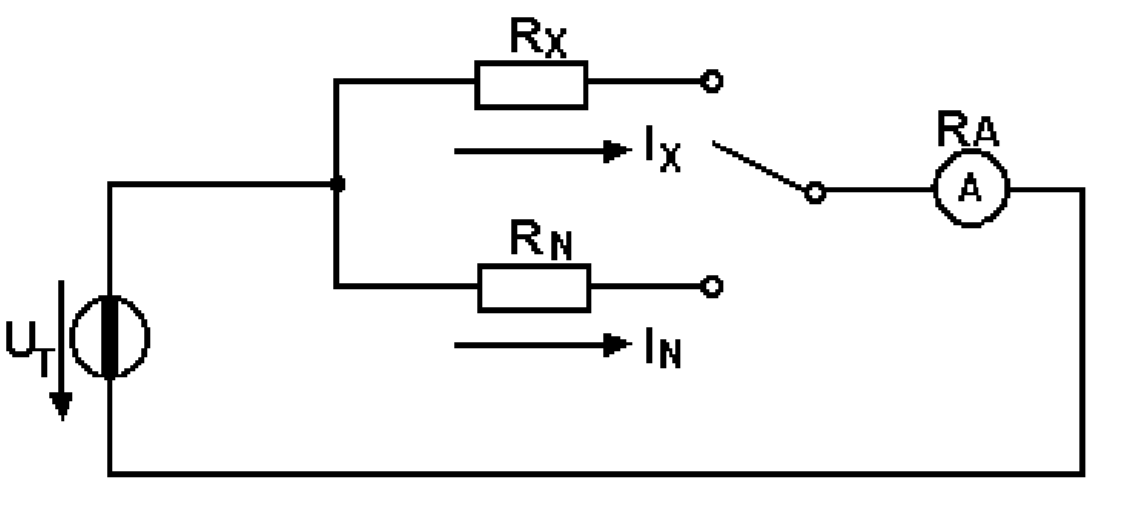
\includegraphics[scale=0.2]{teljes/aram_ossze.png}
		\caption{Áram összehasonlító módszer}
		\end{figure}
		\\\\Határadatok: Áramkorlát $I = 3mA$, feszültségkorlát:$$
		P= U*I$$
		$$U_{max} = \sqrt{P*R} = \sqrt{0,25 * 100 k\Omega} = 158V$$
		$$U_T = \frac{U_{max}}{5} = 30 V $$
		\\\\Mért értékek:\\\\
		\begin{tabular}{|c|c|c|}
		\hline 
		$R_x$ & $R_{11}$ & $R_{15}$ \\ 
		\hline 
		$I_N$ &  &  \\ 
		\hline 
		$I_X$ &  &  \\ 
		\hline 
		$R_{valodi}$ &   &  \\ 
		\hline 
		\end{tabular}
		$$R_X = R_N * \frac{I_N}{I_X}$$ 
		Hibaszámítás (Maxwell):
		\\\\ $$$$ $$$$
		\newpage
		\subsection{Két- ill. négyvezetékes módszer segítségével határozza meg a 4. sz
mérőpanelen található R3 =$ 0,5\Omega$ névleges értékű ellenállást! A mért és a
számított eredményeket foglalja össze táblázatba A méréseknél az elérhető
legnagyobb pontosságra törekedjék!}
		Mérendő objektum:\\\\
		\begin{figure}[hbtp]
		\centering
		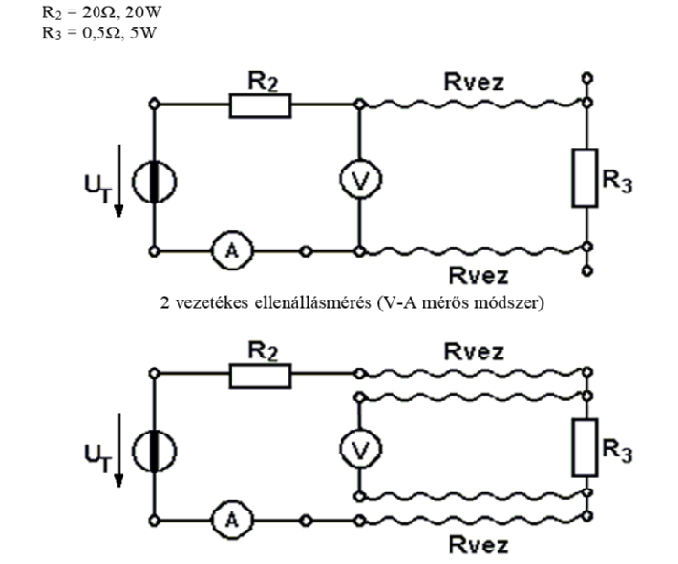
\includegraphics[scale=0.5]{teljes/ket_negy_vez.png}
		\caption{4 vezetékes ellenállásmérés}
		\end{figure}
		
		Határadatok:
		$$I = \sqrt{\frac{P_{R2}}{R_2}} I = \sqrt{\frac{20W}{20\Omega}} = 1 A$$
		$$U_T = I * \left(R2 + R3\right) = 1A * \left(20\Omega + 0,5\Omega\right) = 20,5 V$$\begin{tabular}{|c|c|c|c|}
		\hline 
		Módszer & I & U & R \\ 
		\hline 
		Kétvezetékes rövid &  &  &  \\ 
		\hline 
		Kétvezetékes hosszú &  & &  \\ 
		\hline 
		Négyvezetékes rövid &  &  &  \\ 
		\hline 
		Négyvezetékes hosszú &  &  &  \\ 
		\hline 
		\end{tabular} 
\end{document}